\chapter{Problem Formulation}
Given a weighted graph $\mathcal{G}=(V, E, w)$ and an objective function $F:2^E \rightarrow \mathbb{R}^+$, where $V$ is a set of vertex, $E$ is a set of edges and $w:E \rightarrow \mathbb{R}^+$ is a distance function, the goal is to find a subset $S \subseteq E$ that maximizes environmental coverage and balances robot workloads subject to a constraint.
The objective function $F(S)=f(S)+\lambda \mathcal{B}(S)$ \cite{li2024mrsis} is defined as a linear combination of a coverage function $f$ and a balancing function $\mathcal{B}$, where $\lambda \in [0,1]$ is the weight of the balancing function\footnote{Both $f$ and $\mathcal{B}$ functions are normalized.}.
In 3D environments, the coverage function is defined by calculating the ratio of the number of covered voxels to the total number of environmental voxels.

Two variant formulations with known world maps are considered: Multi-robot search with independence system (MRSIS) \cite{li2024mrsis} and Multi-robot search with matroid (MRSM). \\

\section{Multi-robot search with independence system (MRSIS)}
\begin{problem} \label{prob:objective-IS}
    (MRSIS) \cite{li2024mrsis} Given an objective function $F$, a set of independence system $\mathit{\mathbb{I}} = \{I_G , I_C\}$, the number of robots $n \in \mathbb{N}^+$, and a set of routing constraints for each robot $l = \{l_i \in \mathbb{R}^+\}_{i=1}^n$, find a subset $S \subseteq E$ that maximizes $F$ under an intersection of independence systems
    \begin{equation} \label{eq:objective-IS}
        \begin{aligned}
            \max_{S} \quad & F(S) \\
            \textrm{s.t.} \quad & S \in \bigcap_{I \in \mathit{\mathbb{I}}} I,
        \end{aligned}
\end{equation}
\end{problem}

The intersection system $\bigcap_{I \in \mathit{\mathbb{I}}} I$ is defined as an intersection of all elements in the set of independence systems.
$\mathit{\mathbb{I}} = \{I_G , I_C\}$ is defined as a set of independence systems, where $I_G=(E, \mathcal{I}_G)$ models the robots' routing constraint and $I_C=(E, \mathcal{I}_C)$ models the cluster constraint.\\


The following theorems and corollaries prove that the routing and clustering constraints are $k$-independence systems.
Then, the theoretical performance guarantee of MRSIS \cite{li2024mrsis} is provided.


\begin{theorem} \label{thm:general-routing} (Routing constraint of a $k$-independence system)
The routing constraint for multiple robots $I_G=(E, \mathcal{I}_G)$ is a $k_G$-independence system, where $k_G > 1$. The independent set is defined as $\mathcal{I}_G=\{S \subseteq E : c(S \cap X_i) \leq l_i , \forall i\in \{1,...,n\}\}$, where $c:2^E \rightarrow \mathbb{R}^+$ is a routing cost function (e.g., TSP or MST solver), $X_i \subseteq S$ is the set of $i^{th}$ cluster and $l_i$ is a routing budget.
\end{theorem}
\begin{proof}
To prove that $I_G$ is an independence system, two properties described in Def. \ref{def:independence-system} must hold.

\textbf{(Non-emptiness property)} Consider a set $B_1=\emptyset$.
Let $A=\{1,...,n\}$ and $m_i=c(B_1 \cap X_i), \forall i\in A$ be the routing costs of the $i$-th cluster and $X_i$ be a set of cluster $i$. Since $B_1$ is an empty set, it implies that $m_i=0, \forall i\in A$. Thus, $B_1$ belongs to the independent set $\mathcal{I}_G$.

\textbf{(Downward closure property)} Consider a set $B_1\subseteq E$ and $B_1 \in \mathcal{I}_G$. Let $m_i=c(B_1 \cap X_i), \forall i\in A$ be the routing costs of the $i$-th cluster and $X_i$ be a set of cluster $i$.
Since $B_1 \in \mathcal{I}_G$, this implies that $c(B_1 \cap X_i) \leq l_i, \forall i\in A$. Therefore, $m_i \leq l_i, \forall i\in A$. Let $B_2 \subseteq B_1$ and $n_i=c(B_2 \cap X_i), \forall i\in A$. Since $B_2$ contains edges no more than $B_1$, the routing costs $n_i \leq m_i$. As a result, $n_i \leq m_i \leq l_i$. Therefore, $B_2$ belongs to the independent set $\mathcal{I}_G$.

Since the independent set $\mathcal{I}_G$ satisfies the non-emptiness and downward closure properties, $I_G=(E, \mathcal{I}_G)$ is a $k_G$-independence system. If $I_G$ does not satisfy the exchange property (Def. \ref{def-matroid}), $k_G$ will be greater than 1.

To prove that $k_G > 1$, consider two sets $B_1\in \mathcal{I}$ and $B_2 \in \mathcal{I}$, where $|B_1|>|B_2|$.
Let $s=B_1 \setminus B_2$, $m_i=c(B_1 \cap X_i)\leq l_i, \forall i\in A$ and $n_i=c(B_2 \cap X_i)=l_i, \forall i\in A$. If $X \notin \emptyset$, adding any element $x \in X$ to $B_2$ forms a new set $B_2'$. It is obvious that $B_2' \notin \mathcal{I}$ since $n_i=l_i \leq c(B_2' \cap X_i)$.
Therefore, $I_G$ does not satisfy the exchange property. $k_G$ is greater than 1.
\\
\end{proof}

\begin{corollary} \label{cor:clustering-indep-sys} (Clustering constraint as a $1$-independence system)
Let $E$ be an edge set and $S \subseteq E$ be a subset.
$I_C=(E, \mathcal{I}_C)$ is an $1$-independence system, where $\mathcal{I}_C=\{S \subseteq E : N \geq n \}$, $N$ is the number of clusters, and $n$ is the number of robots.
\end{corollary}
\begin{proof}
Since $I_C$ is a matroid (Thm. \ref{thm:clustering-matroid}) and matroid satisfies the properties of the independence system (Def. \ref{def:independence-system}),
the clustering constraint $I_C$ is an $1$-independence system.
\\
\end{proof}

\begin{theorem}  \label{def:independence-bound}
 (Lower bound of MRSIS\cite{li2024mrsis}) Let $F$ be the coverage and balancing function, $\mathit{\mathbb{I}}$ be a set of $k$-independence systems, $S$ be the solution of maximizing $F$ subject to the intersection of $\mathit{\mathbb{I}}$ via greedy algorithms. The performance of $S$ is
\begin{equation*}
      F(X) \geq \frac{1}{2+k_G} F(\overline{X^{opt}}),
\end{equation*}
where $k_G > 1$ and $\overline{X^{opt}}$ is an approximately optimal solution depending on the TSP or MST solver.
\end{theorem}
\begin{proof}
In Thm. \ref{thm:proposed-obj}, the coverage and balancing function $F$ satisfies the submodularity.
Let $\mathit{\mathbb{I}}=\{I_C, I_G\}$ be a set of $k$-independence systems. In Cor. \ref{cor:clustering-indep-sys}, the clustering constraint $I_C$ is a $1$-independence system. In Thm. \ref{thm:general-routing}, the general multi-robot routing constraint $I_G$ is a $k_G$-independence system.
By Thm. \ref{thm:intersection-k-systems}, the performance of MRSIS \cite{li2024mrsis} achieves $\frac{1}{2+k_G}\overline{OPT}$, where $\overline{OPT}$ is an approximately optimal solution that depends on the routing cost function.
\\
\end{proof}

To improve the performance of MRSIS \cite{li2024mrsis}, the set of independence systems is reformulated into the set of matroids.

\section{Multi-robot search with matroid (MRSM)}

\begin{problem} \label{prob:objective-Mat}
    (MRSM) Given an objective function $F$, a set of matroidal independence systems $\mathit{\mathbb{M}} = \{\mathcal{M}_R , \mathcal{M}_C\}$, the number of robots $n \in \mathbb{N}^+$, and a set of routing constraints for each robot $l = \{l_i \in \mathbb{R}^+\}_{i=1}^n$, find a set $S \subseteq E$ that maximizes $F$ under an intersection of matroidal independence systems
    \begin{equation} \label{eq:objective-Mat}
        \begin{aligned}
            \max_{S} \quad & F(S) \\
            \textrm{s.t.} \quad & S \in \bigcap_{\mathcal{M}\in \mathit{\mathbb{M}}} \mathcal{M},
        \end{aligned}
\end{equation}
\end{problem}

$\mathit{\mathbb{M}} = \{\mathcal{M}_R , \mathcal{M}_C\}$ is defined as a set of matroidal independence systems, where $\mathcal{M}_R=(E, \mathcal{I}_R)$ and $\mathcal{M}_C=(E, \mathcal{I}_C)$ are the robots routing constraint under tree structure and the clustering constraint, respectively.

The routing matroid $\mathcal{M}_R$ constrains the trajectory length of robots while constructing spanning trees.
The independent set $\mathcal{I}_R$ is a subset of $E$ which satisfies:
\begin{enumerate}
    \item $T \subset S$, where $T \subseteq E$ and $S \subseteq E$ are acyclic, and $|T| < |S|$,
    \item $c_{st}(S \cap X_i) \leq l_i , \forall i\in \{1,2,...,n\}$.
\end{enumerate}
where $X_i \subseteq S$ is the set of the $i^{th}$ cluster and $c_{st}:2^E \rightarrow \mathbb{R}^+$ is a routing cost function for a spanning tree.

The clustering matroid $\mathcal{M}_C$ is defined the same as in MRSIS \cite{li2024mrsis}.
The independent set $\mathcal{I}_C$ is defined as
\begin{align*}
    \mathcal{I}_C=\{S \subseteq E : N \geq n \},
\end{align*}
where $N$ is the number of clusters and $n$ is the number of robots. \\

The following Theorems introduce matroid constraints and the theoretical performance guarantee of MRSM.

\begin{theorem} \label{thm:routing-matroid} (Routing constraint under tree structure)
Let $E$ be an edge set and $T$ and $S$ be any subset of $E$. $\mathcal{I}_R$ is the set of subsets, $S\subseteq E$, which satisfies:
\begin{enumerate}
    \item $T \subset S$, where $T$ and $S$ are acyclic and $|T| < |S|$,
    \item $c_{st}(S \cap X_i) \leq l_i , \forall i\in \{1,...,n\}$, where $c_{st}:2^E \rightarrow \mathbb{R}^+$ is a routing cost function for a spanning tree, $X_i \subseteq S$ is the set of $i^{th}$ cluster and $l_i$ is a routing budget.
\end{enumerate}

The routing constraint $\mathcal{M}_R=(E, \mathcal{I}_R)$ is a matroid.
\end{theorem}
\begin{proof}
To prove that $\mathcal{M}_R$ is a matroid, two properties described in Def. \ref{def:matroid} must hold.

\textbf{(Downward closure property)} Consider a set $B_1\subseteq E$ and $B_1 \in \mathcal{I}_R$.
Let $A=\{1,...,n\}$ and $m_i=c_{st}(B_1 \cap X_i), \forall i\in A$ be the routing costs of the $i$-th cluster, and $X_i$ be the set of the $i$-th cluster.
Since $B_1 \in \mathcal{I}_R$, this implies that $B_1$ is a tree (acyclic graph) and $m_i \leq l_i, \forall i\in A$.
Let $B_2 \subseteq B_1$ and $n_i=c_{st}(B_2 \cap X_i), \forall i\in A$.
Since $B_2$ contains edges no more than $B_1$, the routing costs must be $n_i \leq m_i$.
In addition, removing any edge from $B_1$ forms $B_2$ which does not form a cycle.
As a result, $n_i \leq m_i \leq l_i$ and $B_2$ is acyclic.
Therefore, $\mathcal{I}_R$ satisfies the downward closure property.

\textbf{(Exchange property)} Consider two sets $B_1 \in \mathcal{I}_R$ and $B_2\in \mathcal{I}_R$, where $|B_1|>|B_2|$.
Since $B_1$ and $B_2$ satisfy the condition of the independent set and $|B_1|>|B_2|$, it implies that $B_2 \subset B_1$.
Let $m_i=c_{st}(B_1 \cap X_i)$ and $n_i=c_{st}(B_2 \cap X_i), \forall i\in A$.
If $B_2 \subset B_1$, it is clear that $n_i \leq m_i \leq l_i$.
Besides, removing any edge from $B_1$ forms $B_2$, which is acyclic.
Therefore, $\mathcal{I}_R$ satisfies the exchange property.

Since the independent set $\mathcal{I}_R$ satisfies the downward closure properties and the exchange property, $\mathcal{M}_R=(E, \mathcal{I}_R)$ is a matroid.\\
\end{proof}

\begin{definition}
    (Matroidal independence systems of routing and clustering constraints) Given a tree-structured routing constraint $\mathcal{M}_R$ with a set of routing budgets $\{l_i\}_{i=1}^n$ and a clustering constraint $\mathcal{M}_C$ with $n$ robots. A set of matroidal independence systems is defined as $\mathit{\mathbb{M}} = \{\mathcal{M}_R , \mathcal{M}_C\}$.\\
\end{definition}

The routing matroid $\mathcal{M}_R$ constrains the trajectory length of robots via constructing spanning trees while the clustering matroid $\mathcal{M}_C$ divides the ground set into groups for robots.

To illustrate the concept, two cases are illustrated as follows.
Fig. \ref{independent-set} illustrates the intersection system of $\mathcal{M}_R=(E, \mathcal{I}_R)$ and $\mathcal{M}_C=(E, \mathcal{I}_C)$.
Let $E$ be the set of edges between any vertex, $(a,b)\in E$ be an undirected edge, $\mathit{\mathbb{M}}=\{\mathcal{M}_R, \mathcal{M}_C\}$ be the set of matroidal independence systems, $l_i=10$ be the routing constraint and $n=3$ be the minimum number of clusters. In Fig. \ref{independent-set}(a), let $S_A=\{S_1,S_2,S_3\}$, where $S_1=\{(0,4)\},S_2=\{(3,5)\},$ and $S_3=\{(6,7),$$(7,8)\}$. $S_A$ satisfies the intersection system since $S_A$ is acyclic, $|S_A|\geq n$ and $c(S_A \cap S_i) \leq l_i$, where $i=\{1,2,3\}$.
In Fig. \ref{independent-set}(b), let $S_B=\{S_1,S_2\}$, where $S_1=\{(0,4),(4,2),(2,5),(3,5)\}$ and $S_2=\{(6,7),$$(7,8)\}$. $S_B$ does not satisfy the intersection system since $|S_B| < n$ and $c(S_B \cap S_1) > l_i$. \\

\begin{figure}
    \centering
    \begin{subfigure}[b]{0.4\textwidth}
        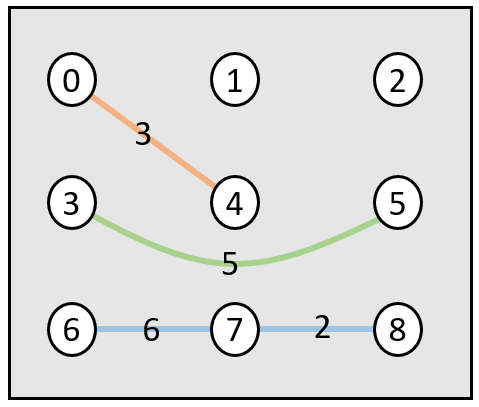
\includegraphics[width=1\textwidth]{mat-1.png}
        \caption{$S_A \in \bigcap_{\mathcal{M}\in \mathit{\mathbb{M}}} \mathcal{M}$}
    \end{subfigure}
    \hfill
    \quad
    \begin{subfigure}[b]{0.4\textwidth}
    \centering
        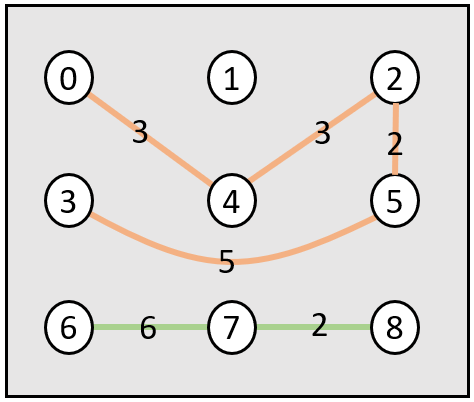
\includegraphics[width=1\textwidth]{mat-2.png}
        \caption{$S_B \not \in \bigcap_{\mathcal{M}\in \mathit{\mathbb{M}}} \mathcal{M}$}
    \end{subfigure}

    \caption{Illustration of the intersection system.
    The vertices and lines represent the subgoals and the distances between two vertices, respectively.
    Each color line denotes a cluster. (a) $S_A$ contains three clusters that satisfy the condition of the intersection system. (b) $S_B$ contains two clusters that violate the condition of the intersection system due to the under-budget of the clustering and the over-budget of routing constraints.
    }
    \label{independent-set}
\end{figure}

\begin{theorem}  \label{def:proposed-bound}
 (Lower bound of the proposed algorithm for MRSM) Let $F$ be the coverage and balancing function, $\mathit{\mathbb{M}}$ be a set of matroidal independence systems, $S$ be the solution of maximizing $F$ subject to the intersection of $\mathit{\mathbb{M}}$ via greedy algorithms. The performance of $S$ is
\begin{equation*}
      F(X) \geq \frac{1}{3} F(\widetilde{X^{opt}}),
\end{equation*}
where $\widetilde{X^{opt}}$ is the optimal solution under tree structure.
\end{theorem}
\begin{proof}
The coverage and balancing function $F$ is submodular (Thm. \ref{thm:proposed-obj}) and each element in $\mathit{\mathbb{M}}$ is a matroid (Thm. \ref{thm:clustering-matroid} and Thm. \ref{thm:routing-matroid}).
By Thm. \ref{thm:intersection-matroid-bound}, the performance of the proposed method is guaranteed to find a solution that achieves $\frac{1}{3}\widetilde{OPT}$, where $\widetilde{OPT}$ is the optimal performance under tree structure.
\end{proof}

